\documentclass[1p]{elsarticle_modified}
%\bibliographystyle{elsarticle-num}

%\usepackage[colorlinks]{hyperref}
%\usepackage{abbrmath_seonhwa} %\Abb, \Ascr, \Acal ,\Abf, \Afrak
\usepackage{amsfonts}
\usepackage{amssymb}
\usepackage{amsmath}
\usepackage{amsthm}
\usepackage{scalefnt}
\usepackage{amsbsy}
\usepackage{kotex}
\usepackage{caption}
\usepackage{subfig}
\usepackage{color}
\usepackage{graphicx}
\usepackage{xcolor} %% white, black, red, green, blue, cyan, magenta, yellow
\usepackage{float}
\usepackage{setspace}
\usepackage{hyperref}

\usepackage{tikz}
\usetikzlibrary{arrows}

\usepackage{multirow}
\usepackage{array} % fixed length table
\usepackage{hhline}

%%%%%%%%%%%%%%%%%%%%%
\makeatletter
\renewcommand*\env@matrix[1][\arraystretch]{%
	\edef\arraystretch{#1}%
	\hskip -\arraycolsep
	\let\@ifnextchar\new@ifnextchar
	\array{*\c@MaxMatrixCols c}}
\makeatother %https://tex.stackexchange.com/questions/14071/how-can-i-increase-the-line-spacing-in-a-matrix
%%%%%%%%%%%%%%%

\usepackage[normalem]{ulem}

\newcommand{\msout}[1]{\ifmmode\text{\sout{\ensuremath{#1}}}\else\sout{#1}\fi}
%SOURCE: \msout is \stkout macro in https://tex.stackexchange.com/questions/20609/strikeout-in-math-mode

\newcommand{\cancel}[1]{
	\ifmmode
	{\color{red}\msout{#1}}
	\else
	{\color{red}\sout{#1}}
	\fi
}

\newcommand{\add}[1]{
	{\color{blue}\uwave{#1}}
}

\newcommand{\replace}[2]{
	\ifmmode
	{\color{red}\msout{#1}}{\color{blue}\uwave{#2}}
	\else
	{\color{red}\sout{#1}}{\color{blue}\uwave{#2}}
	\fi
}

\newcommand{\Sol}{\mathcal{S}} %segment
\newcommand{\D}{D} %diagram
\newcommand{\A}{\mathcal{A}} %arc


%%%%%%%%%%%%%%%%%%%%%%%%%%%%%5 test

\def\sl{\operatorname{\textup{SL}}(2,\Cbb)}
\def\psl{\operatorname{\textup{PSL}}(2,\Cbb)}
\def\quan{\mkern 1mu \triangleright \mkern 1mu}

\theoremstyle{definition}
\newtheorem{thm}{Theorem}[section]
\newtheorem{prop}[thm]{Proposition}
\newtheorem{lem}[thm]{Lemma}
\newtheorem{ques}[thm]{Question}
\newtheorem{cor}[thm]{Corollary}
\newtheorem{defn}[thm]{Definition}
\newtheorem{exam}[thm]{Example}
\newtheorem{rmk}[thm]{Remark}
\newtheorem{alg}[thm]{Algorithm}

\newcommand{\I}{\sqrt{-1}}
\begin{document}

%\begin{frontmatter}
%
%\title{Boundary parabolic representations of knots up to 8 crossings}
%
%%% Group authors per affiliation:
%\author{Yunhi Cho} 
%\address{Department of Mathematics, University of Seoul, Seoul, Korea}
%\ead{yhcho@uos.ac.kr}
%
%
%\author{Seonhwa Kim} %\fnref{s_kim}}
%\address{Center for Geometry and Physics, Institute for Basic Science, Pohang, 37673, Korea}
%\ead{ryeona17@ibs.re.kr}
%
%\author{Hyuk Kim}
%\address{Department of Mathematical Sciences, Seoul National University, Seoul 08826, Korea}
%\ead{hyukkim@snu.ac.kr}
%
%\author{Seokbeom Yoon}
%\address{Department of Mathematical Sciences, Seoul National University, Seoul, 08826,  Korea}
%\ead{sbyoon15@snu.ac.kr}
%
%\begin{abstract}
%We find all boundary parabolic representation of knots up to 8 crossings.
%
%\end{abstract}
%\begin{keyword}
%    \MSC[2010] 57M25 
%\end{keyword}
%
%\end{frontmatter}

%\linenumbers
%\tableofcontents
%
\newcommand\colored[1]{\textcolor{white}{\rule[-0.35ex]{0.8em}{1.4ex}}\kern-0.8em\color{red} #1}%
%\newcommand\colored[1]{\textcolor{white}{ #1}\kern-2.17ex	\textcolor{white}{ #1}\kern-1.81ex	\textcolor{white}{ #1}\kern-2.15ex\color{red}#1	}

{\Large $\underline{12n_{0444}~(K12n_{0444})}$}

\setlength{\tabcolsep}{10pt}
\renewcommand{\arraystretch}{1.6}
\vspace{1cm}\begin{tabular}{m{100pt}>{\centering\arraybackslash}m{274pt}}
\multirow{5}{120pt}{
	\centering
	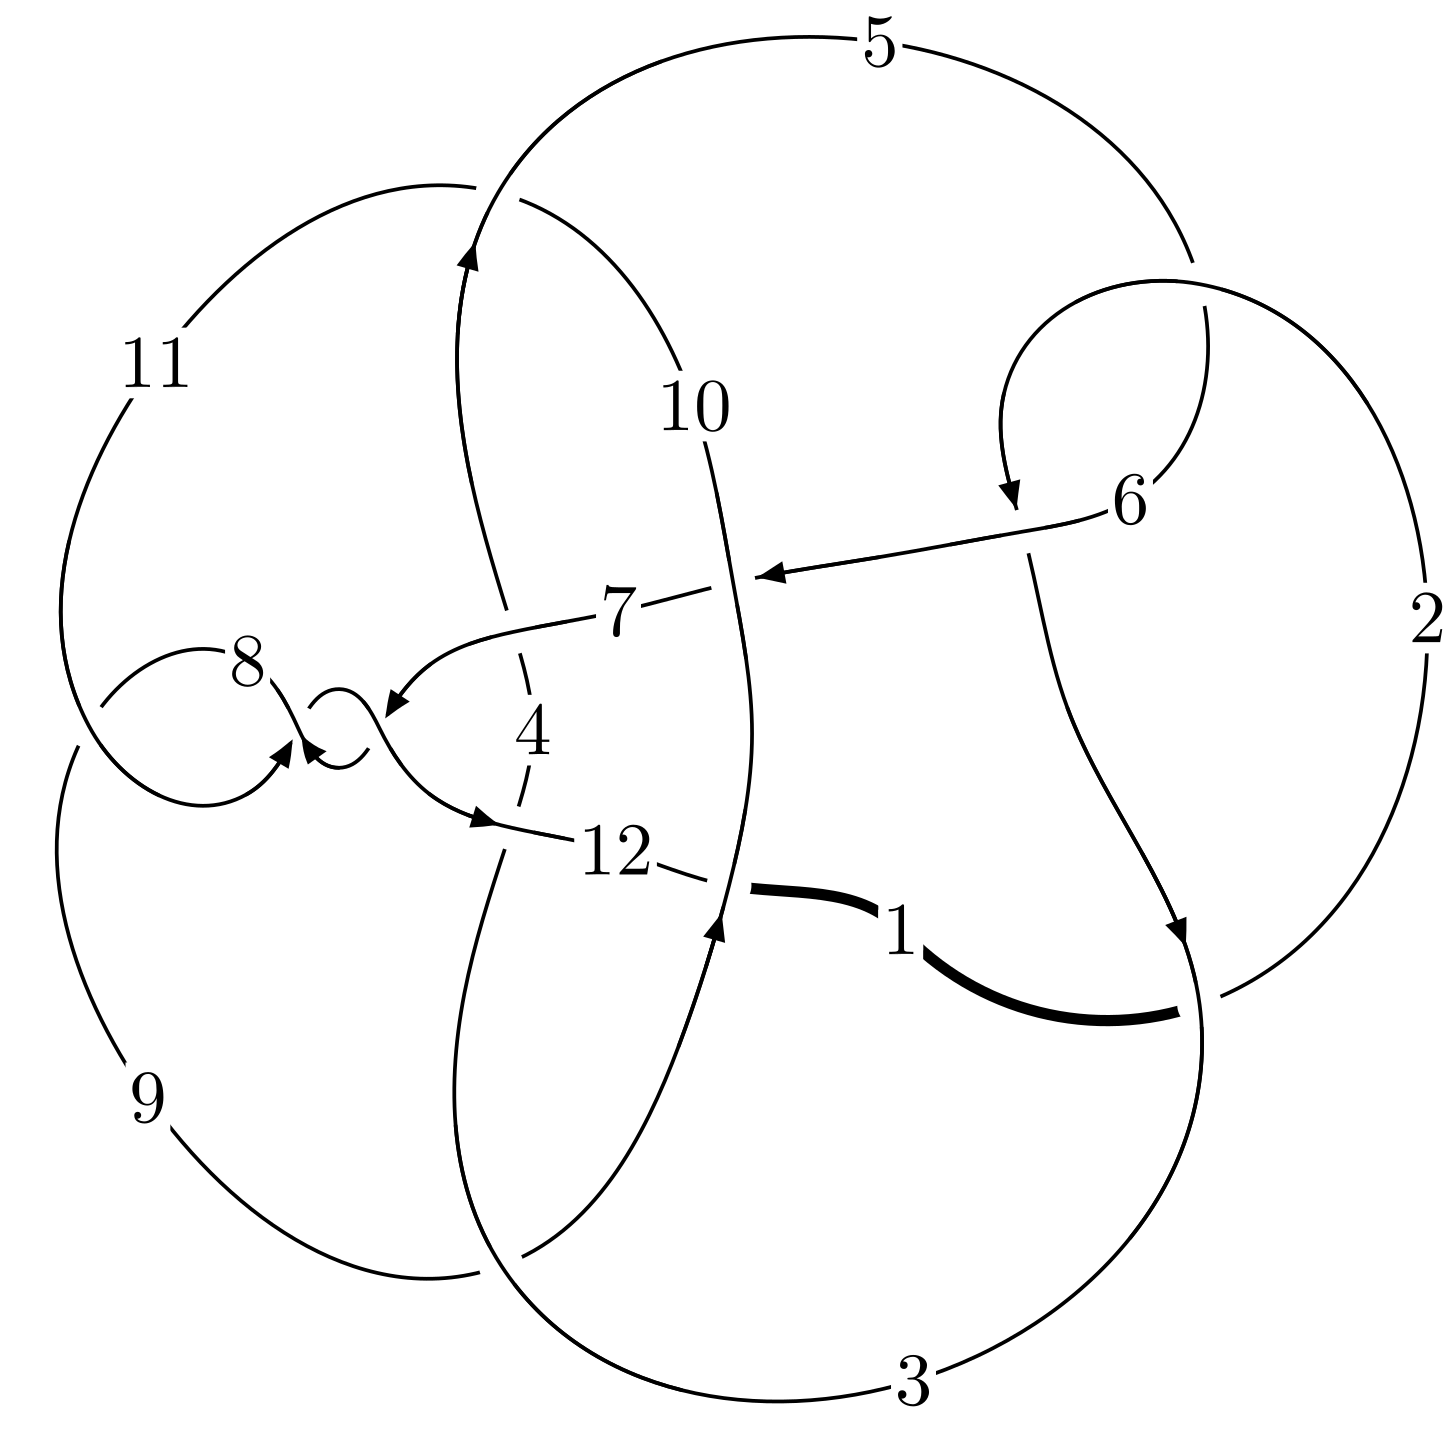
\includegraphics[width=112pt]{../../../GIT/diagram.site/Diagrams/png/2533_12n_0444.png}\\
\ \ \ A knot diagram\footnotemark}&
\allowdisplaybreaks
\textbf{Linearized knot diagam} \\
\cline{2-2}
 &
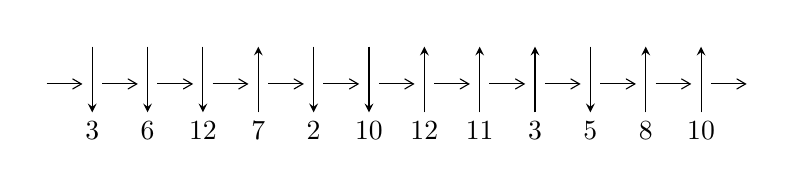
\begin{tikzpicture}[x=20pt, y=17pt]
	% nodes
	\node (C0) at (0, 0) {};
	\node (C1) at (1, 0) {};
	\node (C1U) at (1, +1) {};
	\node (C1D) at (1, -1) {3};

	\node (C2) at (2, 0) {};
	\node (C2U) at (2, +1) {};
	\node (C2D) at (2, -1) {6};

	\node (C3) at (3, 0) {};
	\node (C3U) at (3, +1) {};
	\node (C3D) at (3, -1) {12};

	\node (C4) at (4, 0) {};
	\node (C4U) at (4, +1) {};
	\node (C4D) at (4, -1) {7};

	\node (C5) at (5, 0) {};
	\node (C5U) at (5, +1) {};
	\node (C5D) at (5, -1) {2};

	\node (C6) at (6, 0) {};
	\node (C6U) at (6, +1) {};
	\node (C6D) at (6, -1) {10};

	\node (C7) at (7, 0) {};
	\node (C7U) at (7, +1) {};
	\node (C7D) at (7, -1) {12};

	\node (C8) at (8, 0) {};
	\node (C8U) at (8, +1) {};
	\node (C8D) at (8, -1) {11};

	\node (C9) at (9, 0) {};
	\node (C9U) at (9, +1) {};
	\node (C9D) at (9, -1) {3};

	\node (C10) at (10, 0) {};
	\node (C10U) at (10, +1) {};
	\node (C10D) at (10, -1) {5};

	\node (C11) at (11, 0) {};
	\node (C11U) at (11, +1) {};
	\node (C11D) at (11, -1) {8};

	\node (C12) at (12, 0) {};
	\node (C12U) at (12, +1) {};
	\node (C12D) at (12, -1) {10};
	\node (C13) at (13, 0) {};

	% arrows
	\draw[->,>={angle 60}]
	(C0) edge (C1) (C1) edge (C2) (C2) edge (C3) (C3) edge (C4) (C4) edge (C5) (C5) edge (C6) (C6) edge (C7) (C7) edge (C8) (C8) edge (C9) (C9) edge (C10) (C10) edge (C11) (C11) edge (C12) (C12) edge (C13) ;	\draw[->,>=stealth]
	(C1U) edge (C1D) (C2U) edge (C2D) (C3U) edge (C3D) (C4D) edge (C4U) (C5U) edge (C5D) (C6U) edge (C6D) (C7D) edge (C7U) (C8D) edge (C8U) (C9D) edge (C9U) (C10U) edge (C10D) (C11D) edge (C11U) (C12D) edge (C12U) ;
	\end{tikzpicture} \\
\hhline{~~} \\& 
\textbf{Solving Sequence} \\ \cline{2-2} 
 &
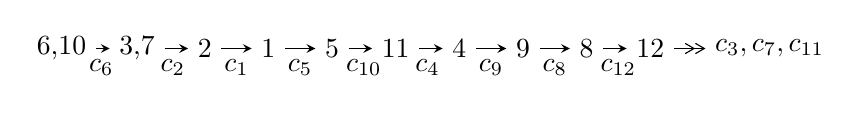
\begin{tikzpicture}[x=23pt, y=7pt]
	% node
	\node (A0) at (-1/8, 0) {6,10};
	\node (A1) at (17/16, 0) {3,7};
	\node (A2) at (17/8, 0) {2};
	\node (A3) at (25/8, 0) {1};
	\node (A4) at (33/8, 0) {5};
	\node (A5) at (41/8, 0) {11};
	\node (A6) at (49/8, 0) {4};
	\node (A7) at (57/8, 0) {9};
	\node (A8) at (65/8, 0) {8};
	\node (A9) at (73/8, 0) {12};
	\node (C1) at (1/2, -1) {$c_{6}$};
	\node (C2) at (13/8, -1) {$c_{2}$};
	\node (C3) at (21/8, -1) {$c_{1}$};
	\node (C4) at (29/8, -1) {$c_{5}$};
	\node (C5) at (37/8, -1) {$c_{10}$};
	\node (C6) at (45/8, -1) {$c_{4}$};
	\node (C7) at (53/8, -1) {$c_{9}$};
	\node (C8) at (61/8, -1) {$c_{8}$};
	\node (C9) at (69/8, -1) {$c_{12}$};
	\node (A10) at (11, 0) {$c_{3},c_{7},c_{11}$};

	% edge
	\draw[->,>=stealth]	
	(A0) edge (A1) (A1) edge (A2) (A2) edge (A3) (A3) edge (A4) (A4) edge (A5) (A5) edge (A6) (A6) edge (A7) (A7) edge (A8) (A8) edge (A9) ;
	\draw[->>,>={angle 60}]	
	(A9) edge (A10);
\end{tikzpicture} \\ 

\end{tabular} \\

\footnotetext{
The image of knot diagram is generated by the software ``\textbf{Draw programme}" developed by Andrew Bartholomew(\url{http://www.layer8.co.uk/maths/draw/index.htm\#Running-draw}), where we modified some parts for our purpose(\url{https://github.com/CATsTAILs/LinksPainter}).
}\phantom \\ \newline 
\centering \textbf{Ideals for irreducible components\footnotemark of $X_{\text{par}}$} 
 
\begin{align*}
I^u_{1}&=\langle 
5.32469\times10^{28} u^{19}-1.94113\times10^{29} u^{18}+\cdots+2.78354\times10^{30} b-8.37086\times10^{31},\\
\phantom{I^u_{1}}&\phantom{= \langle  }-3.59288\times10^{32} u^{19}+1.29989\times10^{33} u^{18}+\cdots+6.03193\times10^{33} a+5.69917\times10^{35},\\
\phantom{I^u_{1}}&\phantom{= \langle  }u^{20}-5 u^{19}+\cdots-5504 u+2167\rangle \\
I^u_{2}&=\langle 
-39167 u^9+24055 u^8+\cdots+90803 b+150893,\;39167 u^9-24055 u^8+\cdots+90803 a-241696,\\
\phantom{I^u_{2}}&\phantom{= \langle  }u^{10}-6 u^8+27 u^6+30 u^5+30 u^4+14 u^3+10 u^2+2 u+1\rangle \\
I^u_{3}&=\langle 
b+1,\;a- u+1,\;u^3-2 u^2+u+1\rangle \\
\\
\end{align*}
\raggedright * 3 irreducible components of $\dim_{\mathbb{C}}=0$, with total 33 representations.\\
\footnotetext{All coefficients of polynomials are rational numbers. But the coefficients are sometimes approximated in decimal forms when there is not enough margin.}
\newpage
\renewcommand{\arraystretch}{1}
\centering \section*{I. $I^u_{1}= \langle 5.32\times10^{28} u^{19}-1.94\times10^{29} u^{18}+\cdots+2.78\times10^{30} b-8.37\times10^{31},\;-3.59\times10^{32} u^{19}+1.30\times10^{33} u^{18}+\cdots+6.03\times10^{33} a+5.70\times10^{35},\;u^{20}-5 u^{19}+\cdots-5504 u+2167 \rangle$}
\flushleft \textbf{(i) Arc colorings}\\
\begin{tabular}{m{7pt} m{180pt} m{7pt} m{180pt} }
\flushright $a_{6}=$&$\begin{pmatrix}1\\0\end{pmatrix}$ \\
\flushright $a_{10}=$&$\begin{pmatrix}0\\u\end{pmatrix}$ \\
\flushright $a_{3}=$&$\begin{pmatrix}0.0595644 u^{19}-0.215502 u^{18}+\cdots+169.749 u-94.4834\\-0.0191292 u^{19}+0.0697361 u^{18}+\cdots-55.2312 u+30.0727\end{pmatrix}$ \\
\flushright $a_{7}=$&$\begin{pmatrix}1\\u^2\end{pmatrix}$ \\
\flushright $a_{2}=$&$\begin{pmatrix}0.0404352 u^{19}-0.145766 u^{18}+\cdots+114.518 u-64.4106\\-0.0191292 u^{19}+0.0697361 u^{18}+\cdots-55.2312 u+30.0727\end{pmatrix}$ \\
\flushright $a_{1}=$&$\begin{pmatrix}-0.0614601 u^{19}+0.224116 u^{18}+\cdots-176.369 u+97.1863\\0.0732431 u^{19}-0.266224 u^{18}+\cdots+209.407 u-116.188\end{pmatrix}$ \\
\flushright $a_{5}=$&$\begin{pmatrix}-0.0367341 u^{19}+0.133131 u^{18}+\cdots-104.597 u+56.9934\\0.0484428 u^{19}-0.177657 u^{18}+\cdots+141.186 u-79.6977\end{pmatrix}$ \\
\flushright $a_{11}=$&$\begin{pmatrix}-0.109966 u^{19}+0.400168 u^{18}+\cdots-316.982 u+175.815\\-0.00769082 u^{19}+0.0267093 u^{18}+\cdots-20.2609 u+10.6953\end{pmatrix}$ \\
\flushright $a_{4}=$&$\begin{pmatrix}-0.153606 u^{19}+0.560090 u^{18}+\cdots-444.350 u+246.211\\-0.164874 u^{19}+0.598489 u^{18}+\cdots-471.899 u+261.395\end{pmatrix}$ \\
\flushright $a_{9}=$&$\begin{pmatrix}0.0266987 u^{19}-0.0960595 u^{18}+\cdots+75.9779 u-40.6092\\-0.115096 u^{19}+0.419259 u^{18}+\cdots-332.122 u+184.578\end{pmatrix}$ \\
\flushright $a_{8}=$&$\begin{pmatrix}0.0291891 u^{19}-0.106960 u^{18}+\cdots+85.6547 u-46.9664\\0.0785887 u^{19}-0.287166 u^{18}+\cdots+225.983 u-125.342\end{pmatrix}$ \\
\flushright $a_{12}=$&$\begin{pmatrix}-0.0614601 u^{19}+0.224116 u^{18}+\cdots-176.369 u+97.1863\\-0.0400440 u^{19}+0.146686 u^{18}+\cdots-115.256 u+64.0732\end{pmatrix}$\\&\end{tabular}
\flushleft \textbf{(ii) Obstruction class $= -1$}\\~\\
\flushleft \textbf{(iii) Cusp Shapes $= -0.0313654 u^{19}+0.114631 u^{18}+\cdots-89.3865 u+39.1345$}\\~\\
\newpage\renewcommand{\arraystretch}{1}
\flushleft \textbf{(iv) u-Polynomials at the component}\newline \\
\begin{tabular}{m{50pt}|m{274pt}}
Crossings & \hspace{64pt}u-Polynomials at each crossing \\
\hline $$\begin{aligned}c_{1}\end{aligned}$$&$\begin{aligned}
&u^{20}+12 u^{19}+\cdots-19 u+4
\end{aligned}$\\
\hline $$\begin{aligned}c_{2},c_{5}\end{aligned}$$&$\begin{aligned}
&u^{20}-2 u^{19}+\cdots-5 u+2
\end{aligned}$\\
\hline $$\begin{aligned}c_{3}\end{aligned}$$&$\begin{aligned}
&u^{20}-5 u^{19}+\cdots-4312 u+581
\end{aligned}$\\
\hline $$\begin{aligned}c_{4}\end{aligned}$$&$\begin{aligned}
&u^{20}- u^{19}+\cdots-622 u+97
\end{aligned}$\\
\hline $$\begin{aligned}c_{6}\end{aligned}$$&$\begin{aligned}
&u^{20}+5 u^{19}+\cdots+5504 u+2167
\end{aligned}$\\
\hline $$\begin{aligned}c_{7},c_{8},c_{11}\end{aligned}$$&$\begin{aligned}
&u^{20}+3 u^{19}+\cdots-71 u+62
\end{aligned}$\\
\hline $$\begin{aligned}c_{9}\end{aligned}$$&$\begin{aligned}
&u^{20}- u^{19}+\cdots-78 u+17
\end{aligned}$\\
\hline $$\begin{aligned}c_{10}\end{aligned}$$&$\begin{aligned}
&u^{20}- u^{19}+\cdots-52 u+17
\end{aligned}$\\
\hline $$\begin{aligned}c_{12}\end{aligned}$$&$\begin{aligned}
&u^{20}+u^{19}+\cdots-294 u+151
\end{aligned}$\\
\hline
\end{tabular}\\~\\
\newpage\renewcommand{\arraystretch}{1}
\flushleft \textbf{(v) Riley Polynomials at the component}\newline \\
\begin{tabular}{m{50pt}|m{274pt}}
Crossings & \hspace{64pt}Riley Polynomials at each crossing \\
\hline $$\begin{aligned}c_{1}\end{aligned}$$&$\begin{aligned}
&y^{20}-8 y^{19}+\cdots-417 y+16
\end{aligned}$\\
\hline $$\begin{aligned}c_{2},c_{5}\end{aligned}$$&$\begin{aligned}
&y^{20}-12 y^{19}+\cdots+19 y+4
\end{aligned}$\\
\hline $$\begin{aligned}c_{3}\end{aligned}$$&$\begin{aligned}
&y^{20}-75 y^{19}+\cdots+153632486 y+337561
\end{aligned}$\\
\hline $$\begin{aligned}c_{4}\end{aligned}$$&$\begin{aligned}
&y^{20}+63 y^{19}+\cdots-66784 y+9409
\end{aligned}$\\
\hline $$\begin{aligned}c_{6}\end{aligned}$$&$\begin{aligned}
&y^{20}-35 y^{19}+\cdots-16056826 y+4695889
\end{aligned}$\\
\hline $$\begin{aligned}c_{7},c_{8},c_{11}\end{aligned}$$&$\begin{aligned}
&y^{20}+37 y^{19}+\cdots+27075 y+3844
\end{aligned}$\\
\hline $$\begin{aligned}c_{9}\end{aligned}$$&$\begin{aligned}
&y^{20}+39 y^{19}+\cdots+6088 y+289
\end{aligned}$\\
\hline $$\begin{aligned}c_{10}\end{aligned}$$&$\begin{aligned}
&y^{20}-5 y^{19}+\cdots-120 y+289
\end{aligned}$\\
\hline $$\begin{aligned}c_{12}\end{aligned}$$&$\begin{aligned}
&y^{20}+47 y^{19}+\cdots+412468 y+22801
\end{aligned}$\\
\hline
\end{tabular}\\~\\
\newpage\flushleft \textbf{(vi) Complex Volumes and Cusp Shapes}
$$\begin{array}{c|c|c}  
\text{Solutions to }I^u_{1}& \I (\text{vol} + \sqrt{-1}CS) & \text{Cusp shape}\\
 \hline 
\begin{aligned}
u &= \phantom{-}0.703317 + 0.600603 I \\
a &= -0.437463 - 0.884492 I \\
b &= -0.924571 + 0.362873 I\end{aligned}
 & -2.03672 + 1.24145 I & -6.74073 - 2.13278 I \\ \hline\begin{aligned}
u &= \phantom{-}0.703317 - 0.600603 I \\
a &= -0.437463 + 0.884492 I \\
b &= -0.924571 - 0.362873 I\end{aligned}
 & -2.03672 - 1.24145 I & -6.74073 + 2.13278 I \\ \hline\begin{aligned}
u &= \phantom{-}0.459645 + 0.743049 I \\
a &= \phantom{-}0.260880 + 0.613052 I \\
b &= \phantom{-}0.118127 - 0.454177 I\end{aligned}
 & \phantom{-}0.254769 - 1.344490 I & \phantom{-}2.10960 + 5.34511 I \\ \hline\begin{aligned}
u &= \phantom{-}0.459645 - 0.743049 I \\
a &= \phantom{-}0.260880 - 0.613052 I \\
b &= \phantom{-}0.118127 + 0.454177 I\end{aligned}
 & \phantom{-}0.254769 + 1.344490 I & \phantom{-}2.10960 - 5.34511 I \\ \hline\begin{aligned}
u &= -0.971034 + 0.814910 I \\
a &= \phantom{-}0.177512 - 0.054619 I \\
b &= \phantom{-}0.759811 + 0.367137 I\end{aligned}
 & \phantom{-}1.28418 - 1.69463 I & \phantom{-}6.51624 + 5.12886 I \\ \hline\begin{aligned}
u &= -0.971034 - 0.814910 I \\
a &= \phantom{-}0.177512 + 0.054619 I \\
b &= \phantom{-}0.759811 - 0.367137 I\end{aligned}
 & \phantom{-}1.28418 + 1.69463 I & \phantom{-}6.51624 - 5.12886 I \\ \hline\begin{aligned}
u &= \phantom{-}1.358840 + 0.009534 I \\
a &= -0.18107 + 1.59414 I \\
b &= \phantom{-}1.34261 - 0.46139 I\end{aligned}
 & \phantom{-}16.5713 + 0.1764 I & -5.92523 - 0.80143 I \\ \hline\begin{aligned}
u &= \phantom{-}1.358840 - 0.009534 I \\
a &= -0.18107 - 1.59414 I \\
b &= \phantom{-}1.34261 + 0.46139 I\end{aligned}
 & \phantom{-}16.5713 - 0.1764 I & -5.92523 + 0.80143 I \\ \hline\begin{aligned}
u &= -1.39927 + 0.25928 I \\
a &= -0.153915 - 1.075640 I \\
b &= -0.150857 + 0.864815 I\end{aligned}
 & -5.96211 - 0.50208 I & -3.53348 + 0.08568 I \\ \hline\begin{aligned}
u &= -1.39927 - 0.25928 I \\
a &= -0.153915 + 1.075640 I \\
b &= -0.150857 - 0.864815 I\end{aligned}
 & -5.96211 + 0.50208 I & -3.53348 - 0.08568 I\\
 \hline 
 \end{array}$$\newpage$$\begin{array}{c|c|c}  
\text{Solutions to }I^u_{1}& \I (\text{vol} + \sqrt{-1}CS) & \text{Cusp shape}\\
 \hline 
\begin{aligned}
u &= \phantom{-}1.35298 + 0.59131 I \\
a &= \phantom{-}0.282108 - 0.480951 I \\
b &= \phantom{-}1.105280 + 0.366189 I\end{aligned}
 & -2.42744 - 4.72916 I & -3.24036 + 7.15543 I \\ \hline\begin{aligned}
u &= \phantom{-}1.35298 - 0.59131 I \\
a &= \phantom{-}0.282108 + 0.480951 I \\
b &= \phantom{-}1.105280 - 0.366189 I\end{aligned}
 & -2.42744 + 4.72916 I & -3.24036 - 7.15543 I \\ \hline\begin{aligned}
u &= -1.33962 + 0.86373 I \\
a &= -0.145047 + 1.067730 I \\
b &= \phantom{-}1.296470 - 0.378610 I\end{aligned}
 & -10.43980 + 3.82524 I & -6.93583 - 2.76644 I \\ \hline\begin{aligned}
u &= -1.33962 - 0.86373 I \\
a &= -0.145047 - 1.067730 I \\
b &= \phantom{-}1.296470 + 0.378610 I\end{aligned}
 & -10.43980 - 3.82524 I & -6.93583 + 2.76644 I \\ \hline\begin{aligned}
u &= \phantom{-}1.73280 + 0.79935 I \\
a &= -0.300874 - 1.047990 I \\
b &= -0.057341 + 0.997519 I\end{aligned}
 & -18.5073 - 4.9976 I & -2.68482 + 1.85210 I \\ \hline\begin{aligned}
u &= \phantom{-}1.73280 - 0.79935 I \\
a &= -0.300874 + 1.047990 I \\
b &= -0.057341 - 0.997519 I\end{aligned}
 & -18.5073 + 4.9976 I & -2.68482 - 1.85210 I \\ \hline\begin{aligned}
u &= -1.90586 + 0.34611 I \\
a &= \phantom{-}0.024972 + 0.827392 I \\
b &= -1.189400 - 0.543552 I\end{aligned}
 & -9.03300 - 5.58421 I & -6.18314 + 4.04952 I \\ \hline\begin{aligned}
u &= -1.90586 - 0.34611 I \\
a &= \phantom{-}0.024972 - 0.827392 I \\
b &= -1.189400 + 0.543552 I\end{aligned}
 & -9.03300 + 5.58421 I & -6.18314 - 4.04952 I \\ \hline\begin{aligned}
u &= \phantom{-}2.50819 + 1.00282 I \\
a &= \phantom{-}0.136951 + 0.755014 I \\
b &= -1.300140 - 0.529897 I\end{aligned}
 & \phantom{-}17.1367 - 10.4420 I & -5.38225 + 4.71177 I \\ \hline\begin{aligned}
u &= \phantom{-}2.50819 - 1.00282 I \\
a &= \phantom{-}0.136951 - 0.755014 I \\
b &= -1.300140 + 0.529897 I\end{aligned}
 & \phantom{-}17.1367 + 10.4420 I & -5.38225 - 4.71177 I\\
 \hline 
 \end{array}$$\newpage\newpage\renewcommand{\arraystretch}{1}
\centering \section*{II. $I^u_{2}= \langle -39167 u^9+24055 u^8+\cdots+90803 b+150893,\;39167 u^9-24055 u^8+\cdots+90803 a-241696,\;u^{10}-6 u^8+\cdots+2 u+1 \rangle$}
\flushleft \textbf{(i) Arc colorings}\\
\begin{tabular}{m{7pt} m{180pt} m{7pt} m{180pt} }
\flushright $a_{6}=$&$\begin{pmatrix}1\\0\end{pmatrix}$ \\
\flushright $a_{10}=$&$\begin{pmatrix}0\\u\end{pmatrix}$ \\
\flushright $a_{3}=$&$\begin{pmatrix}-0.431340 u^{9}+0.264914 u^{8}+\cdots-1.16678 u+2.66176\\0.431340 u^{9}-0.264914 u^{8}+\cdots+1.16678 u-1.66176\end{pmatrix}$ \\
\flushright $a_{7}=$&$\begin{pmatrix}1\\u^2\end{pmatrix}$ \\
\flushright $a_{2}=$&$\begin{pmatrix}1\\0.431340 u^{9}-0.264914 u^{8}+\cdots+1.16678 u-1.66176\end{pmatrix}$ \\
\flushright $a_{1}=$&$\begin{pmatrix}2.92164 u^{9}-0.926676 u^{8}+\cdots+10.7123 u-1.76757\\-1.35298 u^{9}+0.191591 u^{8}+\cdots-5.87905 u-0.570664\end{pmatrix}$ \\
\flushright $a_{5}=$&$\begin{pmatrix}-0.431340 u^{9}+0.264914 u^{8}+\cdots-1.16678 u+2.66176\\1.13732 u^{9}-0.470172 u^{8}+\cdots+3.66644 u-1.67648\end{pmatrix}$ \\
\flushright $a_{11}=$&$\begin{pmatrix}- u^9+6 u^7-27 u^5-30 u^4-30 u^3-14 u^2-10 u-2\\0.926676 u^{9}+0.384426 u^{8}+\cdots+9.61086 u+2.92164\end{pmatrix}$ \\
\flushright $a_{4}=$&$\begin{pmatrix}-1.61557 u^{9}+0.780393 u^{8}+\cdots-4.93171 u+4.07332\\1.20899 u^{9}-0.543143 u^{8}+\cdots+3.81972 u-2.19195\end{pmatrix}$ \\
\flushright $a_{9}=$&$\begin{pmatrix}- u^9+6 u^7-27 u^5-30 u^4-30 u^3-14 u^2-10 u-2\\0.735086 u^{9}+0.0469147 u^{8}+\cdots+7.47556 u+1.56866\end{pmatrix}$ \\
\flushright $a_{8}=$&$\begin{pmatrix}-0.429336 u^{9}-1.35298 u^{8}+\cdots-12.2006 u-6.73772\\-0.234717 u^{9}+0.913527 u^{8}+\cdots+4.86712 u+4.70396\end{pmatrix}$ \\
\flushright $a_{12}=$&$\begin{pmatrix}2.92164 u^{9}-0.926676 u^{8}+\cdots+10.7123 u-1.76757\\-1.73741 u^{9}+0.411198 u^{8}+\cdots-6.94734 u+0.356012\end{pmatrix}$\\&\end{tabular}
\flushleft \textbf{(ii) Obstruction class $= 1$}\\~\\
\flushleft \textbf{(iii) Cusp Shapes $= -\frac{418432}{90803} u^9-\frac{85648}{90803} u^8+\frac{2619224}{90803} u^7+\frac{532096}{90803} u^6-\frac{11982728}{90803} u^5-\frac{14963376}{90803} u^4-\frac{12033384}{90803} u^3-\frac{4718044}{90803} u^2-\frac{2327168}{90803} u-\frac{672892}{90803}$}\\~\\
\newpage\renewcommand{\arraystretch}{1}
\flushleft \textbf{(iv) u-Polynomials at the component}\newline \\
\begin{tabular}{m{50pt}|m{274pt}}
Crossings & \hspace{64pt}u-Polynomials at each crossing \\
\hline $$\begin{aligned}c_{1}\end{aligned}$$&$\begin{aligned}
&(u^5-3 u^4+4 u^3- u^2- u+1)^2
\end{aligned}$\\
\hline $$\begin{aligned}c_{2},c_{5}\end{aligned}$$&$\begin{aligned}
&u^{10}-3 u^8+4 u^6- u^4- u^2+1
\end{aligned}$\\
\hline $$\begin{aligned}c_{3}\end{aligned}$$&$\begin{aligned}
&u^{10}+4 u^9+\cdots+10 u+1
\end{aligned}$\\
\hline $$\begin{aligned}c_{4}\end{aligned}$$&$\begin{aligned}
&u^{10}-2 u^9+u^8-4 u^7+7 u^6+10 u^5-8 u^4+14 u^3+53 u^2+25
\end{aligned}$\\
\hline $$\begin{aligned}c_{6}\end{aligned}$$&$\begin{aligned}
&u^{10}-6 u^8+27 u^6+30 u^5+30 u^4+14 u^3+10 u^2+2 u+1
\end{aligned}$\\
\hline $$\begin{aligned}c_{7},c_{8},c_{11}\end{aligned}$$&$\begin{aligned}
&u^{10}+5 u^8+8 u^6+3 u^4- u^2+1
\end{aligned}$\\
\hline $$\begin{aligned}c_{9},c_{10}\end{aligned}$$&$\begin{aligned}
&(u^2+1)^5
\end{aligned}$\\
\hline $$\begin{aligned}c_{12}\end{aligned}$$&$\begin{aligned}
&u^{10}+u^8-10 u^7- u^6+10 u^5+40 u^4+4 u^3-3 u^2-50 u+25
\end{aligned}$\\
\hline
\end{tabular}\\~\\
\newpage\renewcommand{\arraystretch}{1}
\flushleft \textbf{(v) Riley Polynomials at the component}\newline \\
\begin{tabular}{m{50pt}|m{274pt}}
Crossings & \hspace{64pt}Riley Polynomials at each crossing \\
\hline $$\begin{aligned}c_{1}\end{aligned}$$&$\begin{aligned}
&(y^5- y^4+8 y^3-3 y^2+3 y-1)^2
\end{aligned}$\\
\hline $$\begin{aligned}c_{2},c_{5}\end{aligned}$$&$\begin{aligned}
&(y^5-3 y^4+4 y^3- y^2- y+1)^2
\end{aligned}$\\
\hline $$\begin{aligned}c_{3}\end{aligned}$$&$\begin{aligned}
&y^{10}+12 y^9+\cdots-16 y+1
\end{aligned}$\\
\hline $$\begin{aligned}c_{4}\end{aligned}$$&$\begin{aligned}
&y^{10}-2 y^9+\cdots+2650 y+625
\end{aligned}$\\
\hline $$\begin{aligned}c_{6}\end{aligned}$$&$\begin{aligned}
&y^{10}-12 y^9+\cdots+16 y+1
\end{aligned}$\\
\hline $$\begin{aligned}c_{7},c_{8},c_{11}\end{aligned}$$&$\begin{aligned}
&(y^5+5 y^4+8 y^3+3 y^2- y+1)^2
\end{aligned}$\\
\hline $$\begin{aligned}c_{9},c_{10}\end{aligned}$$&$\begin{aligned}
&(y+1)^{10}
\end{aligned}$\\
\hline $$\begin{aligned}c_{12}\end{aligned}$$&$\begin{aligned}
&y^{10}+2 y^9+\cdots-2650 y+625
\end{aligned}$\\
\hline
\end{tabular}\\~\\
\newpage\flushleft \textbf{(vi) Complex Volumes and Cusp Shapes}
$$\begin{array}{c|c|c}  
\text{Solutions to }I^u_{2}& \I (\text{vol} + \sqrt{-1}CS) & \text{Cusp shape}\\
 \hline 
\begin{aligned}
u &= -0.482881 + 0.629714 I \\
a &= \phantom{-}1.000000 - 0.766826 I \\
b &= \phantom{-0.000000 -}0.766826 I\end{aligned}
 & -2.40108\phantom{ +0.000000I} & -1.48114 + 0. I\phantom{ +0.000000I} \\ \hline\begin{aligned}
u &= -0.482881 - 0.629714 I \\
a &= \phantom{-}1.000000 + 0.766826 I \\
b &= \phantom{-0.000000 } -0.766826 I\end{aligned}
 & -2.40108\phantom{ +0.000000I} & -1.48114 + 0. I\phantom{ +0.000000I} \\ \hline\begin{aligned}
u &= \phantom{-}0.098692 + 0.530370 I \\
a &= \phantom{-}1.82238 + 0.33911 I \\
b &= -0.822375 - 0.339110 I\end{aligned}
 & -0.32910 - 1.53058 I & -0.51511 + 4.43065 I \\ \hline\begin{aligned}
u &= \phantom{-}0.098692 - 0.530370 I \\
a &= \phantom{-}1.82238 - 0.33911 I \\
b &= -0.822375 + 0.339110 I\end{aligned}
 & -0.32910 + 1.53058 I & -0.51511 - 4.43065 I \\ \hline\begin{aligned}
u &= -0.090267 + 0.435818 I \\
a &= \phantom{-}2.20015 - 0.45570 I \\
b &= -1.200150 + 0.455697 I\end{aligned}
 & -5.87256 + 4.40083 I & -4.74431 - 3.49859 I \\ \hline\begin{aligned}
u &= -0.090267 - 0.435818 I \\
a &= \phantom{-}2.20015 + 0.45570 I \\
b &= -1.200150 - 0.455697 I\end{aligned}
 & -5.87256 - 4.40083 I & -4.74431 + 3.49859 I \\ \hline\begin{aligned}
u &= -1.83956 + 0.80797 I \\
a &= -0.200152 + 0.455697 I \\
b &= \phantom{-}1.200150 - 0.455697 I\end{aligned}
 & -5.87256 + 4.40083 I & -4.74431 - 3.49859 I \\ \hline\begin{aligned}
u &= -1.83956 - 0.80797 I \\
a &= -0.200152 - 0.455697 I \\
b &= \phantom{-}1.200150 + 0.455697 I\end{aligned}
 & -5.87256 - 4.40083 I & -4.74431 + 3.49859 I \\ \hline\begin{aligned}
u &= \phantom{-}2.31402 + 1.21207 I \\
a &= \phantom{-}0.177625 + 0.339110 I \\
b &= \phantom{-}0.822375 - 0.339110 I\end{aligned}
 & -0.32910 + 1.53058 I & -0.51511 - 4.43065 I \\ \hline\begin{aligned}
u &= \phantom{-}2.31402 - 1.21207 I \\
a &= \phantom{-}0.177625 - 0.339110 I \\
b &= \phantom{-}0.822375 + 0.339110 I\end{aligned}
 & -0.32910 - 1.53058 I & -0.51511 + 4.43065 I\\
 \hline 
 \end{array}$$\newpage\newpage\renewcommand{\arraystretch}{1}
\centering \section*{III. $I^u_{3}= \langle b+1,\;a- u+1,\;u^3-2 u^2+u+1 \rangle$}
\flushleft \textbf{(i) Arc colorings}\\
\begin{tabular}{m{7pt} m{180pt} m{7pt} m{180pt} }
\flushright $a_{6}=$&$\begin{pmatrix}1\\0\end{pmatrix}$ \\
\flushright $a_{10}=$&$\begin{pmatrix}0\\u\end{pmatrix}$ \\
\flushright $a_{3}=$&$\begin{pmatrix}u-1\\-1\end{pmatrix}$ \\
\flushright $a_{7}=$&$\begin{pmatrix}1\\u^2\end{pmatrix}$ \\
\flushright $a_{2}=$&$\begin{pmatrix}u-2\\-1\end{pmatrix}$ \\
\flushright $a_{1}=$&$\begin{pmatrix}-1\\0\end{pmatrix}$ \\
\flushright $a_{5}=$&$\begin{pmatrix}u-1\\-1\end{pmatrix}$ \\
\flushright $a_{11}=$&$\begin{pmatrix}1\\u^2\end{pmatrix}$ \\
\flushright $a_{4}=$&$\begin{pmatrix}u^2-1\\u^2-2 u-2\end{pmatrix}$ \\
\flushright $a_{9}=$&$\begin{pmatrix}1\\u^2\end{pmatrix}$ \\
\flushright $a_{8}=$&$\begin{pmatrix}1\\u^2\end{pmatrix}$ \\
\flushright $a_{12}=$&$\begin{pmatrix}-1\\- u^2\end{pmatrix}$\\&\end{tabular}
\flushleft \textbf{(ii) Obstruction class $= -1$}\\~\\
\flushleft \textbf{(iii) Cusp Shapes $= -6$}\\~\\
\newpage\renewcommand{\arraystretch}{1}
\flushleft \textbf{(iv) u-Polynomials at the component}\newline \\
\begin{tabular}{m{50pt}|m{274pt}}
Crossings & \hspace{64pt}u-Polynomials at each crossing \\
\hline $$\begin{aligned}c_{1},c_{2},c_{5}\end{aligned}$$&$\begin{aligned}
&(u+1)^3
\end{aligned}$\\
\hline $$\begin{aligned}c_{3},c_{4},c_{9}\\c_{10}\end{aligned}$$&$\begin{aligned}
&u^3+u+1
\end{aligned}$\\
\hline $$\begin{aligned}c_{6}\end{aligned}$$&$\begin{aligned}
&u^3+2 u^2+u-1
\end{aligned}$\\
\hline $$\begin{aligned}c_{7},c_{8},c_{11}\end{aligned}$$&$\begin{aligned}
&u^3
\end{aligned}$\\
\hline $$\begin{aligned}c_{12}\end{aligned}$$&$\begin{aligned}
&u^3-2 u^2+u+1
\end{aligned}$\\
\hline
\end{tabular}\\~\\
\newpage\renewcommand{\arraystretch}{1}
\flushleft \textbf{(v) Riley Polynomials at the component}\newline \\
\begin{tabular}{m{50pt}|m{274pt}}
Crossings & \hspace{64pt}Riley Polynomials at each crossing \\
\hline $$\begin{aligned}c_{1},c_{2},c_{5}\end{aligned}$$&$\begin{aligned}
&(y-1)^3
\end{aligned}$\\
\hline $$\begin{aligned}c_{3},c_{4},c_{9}\\c_{10}\end{aligned}$$&$\begin{aligned}
&y^3+2 y^2+y-1
\end{aligned}$\\
\hline $$\begin{aligned}c_{6},c_{12}\end{aligned}$$&$\begin{aligned}
&y^3-2 y^2+5 y-1
\end{aligned}$\\
\hline $$\begin{aligned}c_{7},c_{8},c_{11}\end{aligned}$$&$\begin{aligned}
&y^3
\end{aligned}$\\
\hline
\end{tabular}\\~\\
\newpage\flushleft \textbf{(vi) Complex Volumes and Cusp Shapes}
$$\begin{array}{c|c|c}  
\text{Solutions to }I^u_{3}& \I (\text{vol} + \sqrt{-1}CS) & \text{Cusp shape}\\
 \hline 
\begin{aligned}
u &= \phantom{-}1.23279 + 0.79255 I \\
a &= \phantom{-}0.232786 + 0.792552 I \\
b &= -1.00000\phantom{ +0.000000I}\end{aligned}
 & -1.64493\phantom{ +0.000000I} & -6.00000\phantom{ +0.000000I} \\ \hline\begin{aligned}
u &= \phantom{-}1.23279 - 0.79255 I \\
a &= \phantom{-}0.232786 - 0.792552 I \\
b &= -1.00000\phantom{ +0.000000I}\end{aligned}
 & -1.64493\phantom{ +0.000000I} & -6.00000\phantom{ +0.000000I} \\ \hline\begin{aligned}
u &= -0.465571\phantom{ +0.000000I} \\
a &= -1.46557\phantom{ +0.000000I} \\
b &= -1.00000\phantom{ +0.000000I}\end{aligned}
 & -1.64493\phantom{ +0.000000I} & -6.00000\phantom{ +0.000000I}\\
 \hline 
 \end{array}$$\newpage
\newpage\renewcommand{\arraystretch}{1}
\centering \section*{ IV. u-Polynomials}
\begin{tabular}{m{50pt}|m{274pt}}
Crossings & \hspace{64pt}u-Polynomials at each crossing \\
\hline $$\begin{aligned}c_{1}\end{aligned}$$&$\begin{aligned}
&((u+1)^3)(u^5-3 u^4+\cdots- u+1)^{2}(u^{20}+12 u^{19}+\cdots-19 u+4)
\end{aligned}$\\
\hline $$\begin{aligned}c_{2},c_{5}\end{aligned}$$&$\begin{aligned}
&((u+1)^3)(u^{10}-3 u^8+\cdots- u^2+1)(u^{20}-2 u^{19}+\cdots-5 u+2)
\end{aligned}$\\
\hline $$\begin{aligned}c_{3}\end{aligned}$$&$\begin{aligned}
&(u^3+u+1)(u^{10}+4 u^9+\cdots+10 u+1)(u^{20}-5 u^{19}+\cdots-4312 u+581)
\end{aligned}$\\
\hline $$\begin{aligned}c_{4}\end{aligned}$$&$\begin{aligned}
&(u^3+u+1)(u^{10}-2 u^9+\cdots+53 u^2+25)\\
&\cdot(u^{20}- u^{19}+\cdots-622 u+97)
\end{aligned}$\\
\hline $$\begin{aligned}c_{6}\end{aligned}$$&$\begin{aligned}
&(u^3+2 u^2+u-1)\\
&\cdot(u^{10}-6 u^8+27 u^6+30 u^5+30 u^4+14 u^3+10 u^2+2 u+1)\\
&\cdot(u^{20}+5 u^{19}+\cdots+5504 u+2167)
\end{aligned}$\\
\hline $$\begin{aligned}c_{7},c_{8},c_{11}\end{aligned}$$&$\begin{aligned}
&u^3(u^{10}+5 u^8+\cdots- u^2+1)(u^{20}+3 u^{19}+\cdots-71 u+62)
\end{aligned}$\\
\hline $$\begin{aligned}c_{9}\end{aligned}$$&$\begin{aligned}
&((u^2+1)^5)(u^3+u+1)(u^{20}- u^{19}+\cdots-78 u+17)
\end{aligned}$\\
\hline $$\begin{aligned}c_{10}\end{aligned}$$&$\begin{aligned}
&((u^2+1)^5)(u^3+u+1)(u^{20}- u^{19}+\cdots-52 u+17)
\end{aligned}$\\
\hline $$\begin{aligned}c_{12}\end{aligned}$$&$\begin{aligned}
&(u^3-2 u^2+u+1)\\
&\cdot(u^{10}+u^8-10 u^7- u^6+10 u^5+40 u^4+4 u^3-3 u^2-50 u+25)\\
&\cdot(u^{20}+u^{19}+\cdots-294 u+151)
\end{aligned}$\\
\hline
\end{tabular}\newpage\renewcommand{\arraystretch}{1}
\centering \section*{ V. Riley Polynomials}
\begin{tabular}{m{50pt}|m{274pt}}
Crossings & \hspace{64pt}Riley Polynomials at each crossing \\
\hline $$\begin{aligned}c_{1}\end{aligned}$$&$\begin{aligned}
&(y-1)^3(y^5- y^4+8 y^3-3 y^2+3 y-1)^2\\
&\cdot(y^{20}-8 y^{19}+\cdots-417 y+16)
\end{aligned}$\\
\hline $$\begin{aligned}c_{2},c_{5}\end{aligned}$$&$\begin{aligned}
&((y-1)^3)(y^5-3 y^4+\cdots- y+1)^{2}(y^{20}-12 y^{19}+\cdots+19 y+4)
\end{aligned}$\\
\hline $$\begin{aligned}c_{3}\end{aligned}$$&$\begin{aligned}
&(y^3+2 y^2+y-1)(y^{10}+12 y^9+\cdots-16 y+1)\\
&\cdot(y^{20}-75 y^{19}+\cdots+153632486 y+337561)
\end{aligned}$\\
\hline $$\begin{aligned}c_{4}\end{aligned}$$&$\begin{aligned}
&(y^3+2 y^2+y-1)(y^{10}-2 y^9+\cdots+2650 y+625)\\
&\cdot(y^{20}+63 y^{19}+\cdots-66784 y+9409)
\end{aligned}$\\
\hline $$\begin{aligned}c_{6}\end{aligned}$$&$\begin{aligned}
&(y^3-2 y^2+5 y-1)(y^{10}-12 y^9+\cdots+16 y+1)\\
&\cdot(y^{20}-35 y^{19}+\cdots-16056826 y+4695889)
\end{aligned}$\\
\hline $$\begin{aligned}c_{7},c_{8},c_{11}\end{aligned}$$&$\begin{aligned}
&y^3(y^5+5 y^4+8 y^3+3 y^2- y+1)^2\\
&\cdot(y^{20}+37 y^{19}+\cdots+27075 y+3844)
\end{aligned}$\\
\hline $$\begin{aligned}c_{9}\end{aligned}$$&$\begin{aligned}
&((y+1)^{10})(y^3+2 y^2+y-1)(y^{20}+39 y^{19}+\cdots+6088 y+289)
\end{aligned}$\\
\hline $$\begin{aligned}c_{10}\end{aligned}$$&$\begin{aligned}
&((y+1)^{10})(y^3+2 y^2+y-1)(y^{20}-5 y^{19}+\cdots-120 y+289)
\end{aligned}$\\
\hline $$\begin{aligned}c_{12}\end{aligned}$$&$\begin{aligned}
&(y^3-2 y^2+5 y-1)(y^{10}+2 y^9+\cdots-2650 y+625)\\
&\cdot(y^{20}+47 y^{19}+\cdots+412468 y+22801)
\end{aligned}$\\
\hline
\end{tabular}
\vskip 2pc
\end{document}